% automatically generated document using lt2circuiTikz
\documentclass[tikz,margin={2pt 2pt 2pt 2pt}]{standalone}
\usepackage[compatibility,siunitx,  americanvoltages, americancurrents, europeanresistors, europeaninductors, americanports,%
  straightlabels, fetbodydiode, straightvoltages]{circuitikz}
\usepackage{tikz,amsmath, amssymb,bm,color,pgfkeys,siunitx,ifthen,ulem}
\usepackage{pgfplots}
\pgfplotsset{compat=1.14}
\usetikzlibrary{shapes,arrows}
%\usepackage{agaramondc}					% Adobe Garamond, custom shape
%\renewcommand{\shapedefault}{rtl} % rtl: roman tabular lining

\input{latex_ext}

\usetikzlibrary{backgrounds,calc,positioning}

\usetikzlibrary{circuits.ee.IEC}
\usetikzlibrary{arrows}


% sym32a style

\ctikzset{tripoles/mos style/arrows}
\ctikzset{
	/tikz/circuitikz/quadpoles/coupler/width=1,%1.3
	/tikz/circuitikz/quadpoles/coupler/height=0.952,%1.3
	/tikz/circuitikz/quadpoles/coupler2/width=1,%1.3
	/tikz/circuitikz/quadpoles/coupler2/height=0.952,%1.3
	/tikz/circuitikz/quadpoles/transformer/width=1.425,%1.5
	/tikz/circuitikz/quadpoles/transformer/height=1.425,%1.5
	/tikz/circuitikz/quadpoles/transformer core/width=1.425,%1.5
	/tikz/circuitikz/quadpoles/transformer core/height=1.425,%1.5
	/tikz/circuitikz/quadpoles/gyrator/width=1.425,%1.5
	/tikz/circuitikz/quadpoles/gyrator/height=1.425,%1.5
	%/tikz/circuitikz/monopoles/tlinestub/width=0.1875,%0.25 no effect!
	/tikz/circuitikz/tripoles/american and port/height=0.95,%.8
	/tikz/circuitikz/tripoles/american nand port/height=0.95,%.8
	/tikz/circuitikz/tripoles/american or port/height=0.95,%.8
	/tikz/circuitikz/tripoles/american nor port/height=0.95,%.8
	/tikz/circuitikz/tripoles/american xor port/height=0.95,%.8
	/tikz/circuitikz/tripoles/american xnor port/height=0.95,%.8
	/tikz/circuitikz/bipoles/tline/height=0.4,%0.3
%	/tikz/circuitikz/bipoles/tline/width=1.2,%0.8
	/tikz/circuitikz/bipoles/diode/height=0.375,%
	/tikz/circuitikz/bipoles/diode/width=0.375,%
	/tikz/circuitikz/bipoles/varcap/height=0.375,%
	/tikz/circuitikz/bipoles/varcap/width=0.375,%
	/tikz/circuitikz/tripoles/triac/height=1.05,%
	/tikz/circuitikz/tripoles/triac/width=0.952,%
	/tikz/circuitikz/tripoles/thyristor/height=1.05,%
	/tikz/circuitikz/tripoles/thyristor/width=0.952,%
	/tikz/circuitikz/tripoles/op amp/height=0.952,%
	/tikz/circuitikz/tripoles/op amp/width=1.2,%
	/tikz/circuitikz/tripoles/op amp/font=\footnotesize,
	/tikz/circuitikz/tripoles/gm amp/height=0.952,% 1.7
	/tikz/circuitikz/tripoles/gm amp/width=1.2,% 1.4
	%	/tikz/circuitikz/tripoles/gm amp/font=\footnotesize,
	/tikz/circuitikz/tripoles/plain amp/height=0.952,% 1.7
	/tikz/circuitikz/tripoles/plain amp/width=1.2,% 1.4
	/tikz/circuitikz/bipoles/resistor/voltage/straight label distance/.initial=.8,
	/tikz/circuitikz/bipoles/generic/voltage/straight label distance/.initial=.8,
	/tikz/circuitikz/bipoles/inductor/voltage/straight label distance/.initial=.8,
	/tikz/circuitikz/bipoles/fullgeneric/voltage/straight label distance/.initial=.8,
	/tikz/circuitikz/bipoles/capacitor/voltage/straight label distance/.initial=1.0,
	/tikz/circuitikz/bipoles/thickness=1.6,
}
\ctikzset{v/.append style={/tikz/european voltages}}

\definecolor{netlabelcolor}{rgb}{0, 0, 0}
\definecolor{lttotitextcolor}{rgb}{0, 0.4, 0}
\definecolor{lttotidrawcolor}{rgb}{0, 0, 0}
\definecolor{netcolor}{rgb}{0, 0, 0}

\pgfkeys{/lt2ti/netlabel/font/.initial= \small}
\pgfkeys{/lt2ti/text/font/.initial= \small}

\pgfkeys{/lt2ti/Net/.style= {netcolor}}
\tikzstyle{dashdotdotted}=[dash pattern=on 3pt off 2pt on \the\pgflinewidth off 2pt on \the\pgflinewidth off 2pt]

\pgfkeys{/lt2ti/VArrow/.style= {->,>=latex}}
\pgfkeys{/lt2ti/SArrow/.style= {->,>=angle 90}}

\begin{document}%
	%\centering%
		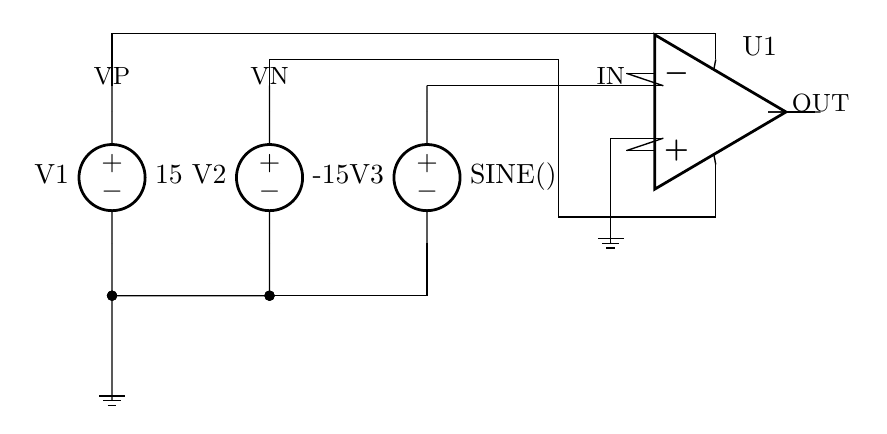
\begin{tikzpicture}[circuit ee IEC, scale=0.6666666667,line width=.5pt]% default: 0.4
	%\tikzstyle{every node}=[font=\small];%
	%\node [draw] at (0.0,0.0) {\pgfkeysvalueof{/tikz/circuitikz/tripoles/op amp/font}};
\draw [/lt2ti/Net](-0.5,-7.0)to[*short,-, color=netcolor] (-0.5,-7.0);% wire w4_w3_w6 start
\draw [/lt2ti/Net](11.0,-6.5)to[*short,-, color=netcolor] (11.0,-6.5);% wire w4_w3_w6 end
\draw [/lt2ti/Net](-0.5,-7.0) --  (-0.5,-6.0) --  (11.0,-6.0) -- (11.0,-6.5); % wire w4_w3_w6 polyline 
\draw [/lt2ti/Net](10.0,-7.0)to[*short,-, color=netcolor] (10.0,-7.0);% wire w8_w9 start
\draw [/lt2ti/Net](5.5,-7.0)to[*short,-, color=netcolor] (5.5,-7.0);% wire w8_w9 end
\draw [/lt2ti/Net](10.0,-7.0) --  (9.0,-7.0) -- (5.5,-7.0); % wire w8_w9 polyline 
\draw [/lt2ti/Net](-0.5,-7.5)to[*short,-, color=netcolor] (-0.5,-7.0);% wire w10
\draw [/lt2ti/Net](2.5,-7.5)to[*short,-, color=netcolor] (2.5,-7.0);% wire w11
\draw [/lt2ti/Net](5.5,-7.5)to[*short,-, color=netcolor] (5.5,-7.0);% wire w12
\draw [/lt2ti/Net](13.0,-7.5)to[*short,-, color=netcolor] (12.0,-7.5);% wire w13
\draw [/lt2ti/Net](10.0,-8.0)to[*short,-, color=netcolor] (10.0,-8.0);% wire w14_w18 start
\draw [/lt2ti/Net](9.0,-10.0)to[*short,-, color=netcolor] (9.0,-10.0);% wire w14_w18 end
\draw [/lt2ti/Net](10.0,-8.0) --  (9.0,-8.0) -- (9.0,-10.0); % wire w14_w18 polyline 
\draw [/lt2ti/Net](11.0,-8.5)to[*short,-, color=netcolor] (11.0,-8.5);% wire w16_w17_w7_w5_w15 start
\draw [/lt2ti/Net](2.5,-7.0)to[*short,-, color=netcolor] (2.5,-7.0);% wire w16_w17_w7_w5_w15 end
\draw [/lt2ti/Net](11.0,-8.5) --  (11.0,-9.5) --  (8.0,-9.5) --  (8.0,-6.5) --  (2.5,-6.5) -- (2.5,-7.0); % wire w16_w17_w7_w5_w15 polyline 
\draw [/lt2ti/Net](-0.5,-11.0)to[*short,*-, color=netcolor] (-0.5,-10.0);% wire w19
\draw [/lt2ti/Net](2.5,-11.0)to[*short,*-, color=netcolor] (2.5,-10.0);% wire w20
\draw [/lt2ti/Net](2.5,-11.0)to[*short,*-*, color=netcolor] (-0.5,-11.0);% wire w21
\draw [/lt2ti/Net](5.5,-10.0)to[*short,-, color=netcolor] (5.5,-10.0);% wire w22_w23 start
\draw [/lt2ti/Net](2.5,-11.0)to[*short,-*, color=netcolor] (2.5,-11.0);% wire w22_w23 end
\draw [/lt2ti/Net](5.5,-10.0) --  (5.5,-11.0) -- (2.5,-11.0); % wire w22_w23 polyline 
\draw [/lt2ti/Net](-0.5,-13.0)to[*short,-*, color=netcolor] (-0.5,-11.0);% wire w24
 \draw (-0.5, -13.0) node[ground, xscale=1, yscale=1, rotate=270, ] (undefined) {};%  (undefined)++(0.0,0.0) node {undefined }; % component "circuiTikz\gnd" "undefined" 
 \draw (9.0, -10.0) node[ground, xscale=1, yscale=1, rotate=270, ] (undefined) {};%  (undefined)++(0.0,0.0) node {undefined }; % component "circuiTikz\gnd" "undefined" 
 \draw (11.08863, -7.5) node[op amp, xscale=1, rotate=0, ] (U1) {}  (U1)++(1*0.75,  1*1.25) node {U1 }; % component "OpAmps/ADA4817" "U1" 
 \draw (11.0,-6.5) to [*short, -] (U1.up);   \draw (11.0,-8.5) to [*short, -] (U1.down); % supply % component "OpAmps/ADA4817" "U1" 
 \draw (10.0,-8.0) to [*short, -] (U1.+);   \draw (10.0,-7.0) to [*short, -] (U1.-); \draw (12.0,-7.5) to [*short, -] (U1.out); % in/out % component "OpAmps/ADA4817" "U1" 
  \draw (-0.5, -7.5) to[*V, l_=V1, a^=15,, -, ] (-0.5,-10.0){}; % component "voltage" "V1" 
  \draw (2.5, -7.5) to[*V, l_=V2, a^=-15,, -, ] (2.5,-10.0){}; % component "voltage" "V2" 
  \draw (5.5, -7.5) to[*V, l_=V3, a^=SINE(),, -, ] (5.5,-10.0){}; % component "voltage" "V3" 
  \node (OUT) [] at (13.0,-7.5) {};% label mark % label "" "OUT" lbl27 
  \node (OUTtxt) [ netlabelcolor, above= -0.24cm of OUT] {{\pgfkeysvalueof{/lt2ti/netlabel/font}OUT}}; % label "" "OUT" lbl27 
  \node (VP) [] at (-0.5,-7.0) {};% label mark % label "" "VP" lbl29 
  \node (VPtxt) [ netlabelcolor, above= -0.24cm of VP] {{\pgfkeysvalueof{/lt2ti/netlabel/font}VP}}; % label "" "VP" lbl29 
  \node (VN) [] at (2.5,-7.0) {};% label mark % label "" "VN" lbl30 
  \node (VNtxt) [ netlabelcolor, above= -0.24cm of VN] {{\pgfkeysvalueof{/lt2ti/netlabel/font}VN}}; % label "" "VN" lbl30 
  \node (IN) [] at (9.0,-7.0) {};% label mark % label "" "IN" lbl31 
  \node (INtxt) [ netlabelcolor, above= -0.24cm of IN] {{\pgfkeysvalueof{/lt2ti/netlabel/font}IN}}; % label "" "IN" lbl31 

	\end{tikzpicture}
\end{document}
